\section{Identifying the PGFs}

G(z,t), the probability generating function, is a powerful tool for understanding the behaviour of the system and its probable outcomes. Because it can be written as a polynomial sum in which each coefficient is the probability of the process being in a specific state at a given time, valuable information on the process can be extracted. \par
As,
$$G(z,t) = p_0(t) + p_1(t)z + p_2(t)z^2 + p_3(t)z^3 + \dots,$$
The mean, $J(t)$ can be found with $\partial_zG(z,t)|_{z=1}$:
$$\mean{\xt} = p_1(t) + 2p_2(t) + 3p_3(t) + \dots;$$
Individual state-probabilities can be extracted in the following way. Differentiate with respect to $z$, $n$ times,
$$\pdxn{G(z,t)}{z}{n} =  n! \cdot p_n(t) + (n+1)! \cdot p_{n+1}(t) z + \frac{(n+2)!}{2} \cdot p_{n+2}(t) z^2 + \dots,$$
then evaluate at $z=0$ and divide by $n!$:
\begin{equation}
\label{stateFormula}
\frac{1}{n!}\cdot\pdxn{G(z,t)}{z}{n}\bigg|_{z=0} = p_n(t).
\end{equation}
In this way the full dynamic distribution of the system can be elucidated.

Though to do this, we must first obtain the explicit formula $G(z,t)$. There will be some difference between the two cases, but the process is similar --- both (\ref{catEq1}) and (\ref{killEq1}) can be solved with the method of characteristics. 


\subsection{Method of characteristics}

Generally, first order, linear PDEs of the type we are dealing can be solved as a family of ODEs. The method begins by introducing a change of variables $(z,t)\to(s,\tau)$;
$$G(z,t)\equiv G\lrb{z(s, \tau),t(s,\tau)} = G(s, \tau).$$
It proceeds by seeking solutions on characteristic lines of constant $s$: $G(\tau)$. An initial curve must be fixed, from which these solutions will progress. The selection is somewhat arbitrary; many options will work, though a good choice can keep the analysis more simple. There are some hard conditions. For example, the initial line must not be parallel in the $s,$ $\tau$ space to the progressing solutions. In cases such as ours, it is often appropriate to use
\begin{align}
\label{ICs}
z(s,0) = s&& t(s,0) = 0
\end{align}

\begin{figure}[H]
\centering
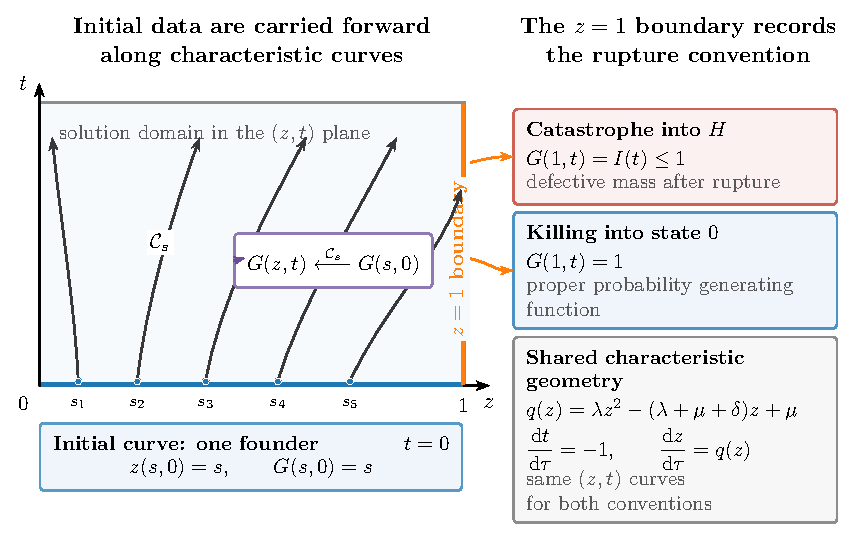
\includegraphics[width=0.95\textwidth]{figures/N4a_1_pgf_characteristics.pdf}
\caption{Method of characteristics for the single-cell \pgf. The initial data
$z(s,0)=s$ and $G(s,0)=s$ are carried along curves generated by
$\dd t/\dd\tau=-1$ and $\dd z/\dd\tau=q(z)$, where
$q(z)=\lambda z^2-(\lambda+\mu+\delta)z+\mu$. The condition at $z=1$
supplies the rupture bookkeeping: $G(1,t)=I(t)$ under catastrophe, whereas
$G(1,t)=1$ when rupture is counted in state $0$. Thus the solution is fixed by
characteristic transport and the stated data rather than by a guessed ansatz.}
\label{fig:N4a_1}
\end{figure}

\subsubsection*{Catastrophe}
Assuming the probability generating function changes with only  one variable --- $G(\tau(z, t))$ --- we can write down the characteristic equations as ODEs. First, consider
\begin{equation*}
\dda{G}{\tau} =  \lrbc{\dda{t}{\tau}}  \pdx{G}{t}+ \lrbc{\dda{z}{\tau} }\pdx{G}{z}.
\end{equation*}
Comparing with the catastrophe equation, (\ref{catEq1}), there is a similarity,
$$0=  \lrbc{- 1}\pdx{G}{t} + \lrbc{\lambda z^2 -( \lambda + \mu + \delta)z + \mu} \pdx{G}{z},$$
and we can extract the three characteristic ODEs:
\begin{align*}
\label{Char1}
\dda{G}{\tau} = 0,&& \dda{t}{\tau} = -1, && \dda{z}{\tau} = \lambda z^2 - (\lambda + \mu + \delta)z + \mu.
\end{align*}
The first of these, which will differ in the killing case, tells us that  
$$G = \phi{(s)},$$
$\phi$ constant on curves of unchanging $s$.\par
In both cases, the initial condition on $G$ will be $$G(z, 0) = z$$ because starting with a single individual means $p_1(0) =1$ and $p_{i\neq1}(0) = 0$. Therefore, $G = \phi{(s)}$ in conjunction with our choice of initial curve, $z(s, 0) = s$, allows $\phi(s)$ to be fixed as $s$;
$$G(s,\tau) = s.$$\par

\noindent
Moving to the second characteristic ODE:
$$\dda{t}{\tau} = -1 \hspace{5pt} \implies \hspace{5pt} t = -\tau +  C_1(s) \text{  (constant for unchanging }s ).$$
Our initial condition, $t(s,0) = 0$ fixes $C_1(s) = 0$, so $t = -\tau$.\par
The remaining characteristic equation with $z$ happens to be the same form as an ODE describing the no-rupture probability, $I(t)$. 
\begin{equation}
\label{char3cat}
\dda{z}{\tau} = \lambda z^2 - (\lambda + \mu + \delta)z + \mu
\end{equation}
What differs is the initial condition. In the case of, $I(t)$, at time 0 it is 1 --- rupture having definitely not occurred; with $z(s,t)$, our chosen initial condition is $z(s, 0) = s$. Hence, the solution to (\ref{char3cat}) is very similar to the formula for $I(t)$, though in places where there is seen a one, here an $s$ is found:
\begin{equation*}
z = \frac{a(s-b) - b(s-a)\ee^{\lambda(a-b) \tau} } {(s-b) - (s-a)\ee^{\lambda(a-b) \tau}}
\end{equation*}
Also, in this it is $\tau$ rather than $t$.\par
Since $G(z, t) = s(z, t)$, we can obtain the final solution in one step: Rearrange the above for $s$, and place $-t$ at each $\tau$. By a happenstance of symmetry, this turns out looking quite the same:
\begin{equation}
\label{s2343}
s = \frac{a(z-b) - b(z-a)\ee^{\lambda(a-b) t} } {(z-b) - (z-a)\ee^{\lambda(a-b) t}}.
\end{equation}
And so we have it, by the somewhat dark art of characteristics, the probability generating function emerges as
\begin{equation*}
G(z,t) = \frac{a(z-b) - b(z-a)\ee^{\lambda(a-b) t} } {(z-b) - (z-a)\ee^{\lambda(a-b) t}}.
\end{equation*}
As will be seen, in obtaining the state probabilities via repeated partial differentiation in $z$, it is advantageous to write the formula as
\begin{equation*}
G(z,t) = \frac{ab(1-\ee^{\lambda(a-b) t}) - z(a-b\ee^{\lambda(a-b) t}) } {  (b-a\ee^{\lambda(a-b) t}) -z(1-\ee^{\lambda(a-b) t})  }
\end{equation*}
For now, let us move on to the modification that is introduced in the killing case. 


\subsubsection*{Killing}

When rupture collapses the process to 0, it may have happened at any positive state.  As we've seen, because of this, the forward Kolmogorov equation describing $p_0(t)$ includes a separate term related to every natural number. Thankfully, these do compress neatly into an expression of the mean, $\mean{\xt} = J(t)$. Hence, in the PDE, (\ref{killEq1}), there is an inhomogeneous term: $\delta J(t)$.\par
Making the same comparison as in the catastrophe case, 

\begin{align*}
\dda{G}{\tau} &=  \lrbc{\dda{t}{\tau}}  \pdx{G}{t}+ \lrbc{\dda{z}{\tau} }\pdx{G}{z}\\
-\delta J(t)&=  \lrbc{- 1}\pdx{G}{t} + \lrbc{\lambda z^2 -( \lambda + \mu + \delta)z + \mu} \pdx{G}{z}
\end{align*}
we see the characteristic equations are largely the same, just that the first picks up this extra component: 
\begin{align*}
\label{Char2}
\dda{G}{\tau} = -\delta J(-\tau),&& \dda{t}{\tau} = -1, && \dda{z}{\tau} = \lambda z^2 - (\lambda + \mu + \delta)z + \mu.
\end{align*}

%last 2 the same

%first:

\noindent
From previous work, we know 
$$-\delta J(t) = \ddt{I(t)}.$$
Simply because $\dd t = -\dd \tau$, it follows that 
$$\delta J(-\tau) = \dda{I(-\tau)}{\tau}.$$
And so, looking to the first characteristic equation, 
$$\dda{G}{\tau} = \dda{I(-\tau)}{\tau},$$
hence,
$$G(s,\tau) = -I(-\tau) + \phi(s).$$
Again, with some $\phi$ stationary for over constant $s$. \par
With the initial condition, $G(z, t=0) = z(s, \tau = 0) = s$,
$$G(s,0) =s= -I(0) + \phi(s),$$
$\phi$ can be fixed: $\phi(s) = 1 + s;$
$$G(s,\tau) = 1 - I(-\tau) + s.$$\par
Identical to the catastrophe case, the final characteristic equation is solved in the same way for the same result, (\ref{s2343}). So finally,
$$G(z,t) = 1 - I(t)  + \frac{ab(1-\ee^{\lambda(a-b) t}) - z(a-b\ee^{\lambda(a-b) t}) } {  (b-a\ee^{\lambda(a-b) t}) -z(1-\ee^{\lambda(a-b) t})  }.$$
And this result makes good sense. With $1 - I(t)$ being the likelihood that the process has made the ``killing'' transition to 0, these two terms stand to complement the probability that state $0$ is reached from individual death (this component arises from the final term).

\subsection{Several founders}
\label{sec:pgf-k-founders}

Both solutions extend to an arbitrary initial condition by the branching
property. If the cell begins with $k$ independent founders, $X_0=k$, then the
$k$ lineages evolve independently and the total count is their sum, so the
\pgf{} is the $k$th power of the single-founder \pgf:
\begin{equation}
G_k(z,t) = \lrb{G(z,t)}^k,
\label{eq:Gk}
\end{equation}
in either rupture convention. In the catastrophe convention this is a
defective \pgf{} with $G_k(1,t)=I(t)^k$; in the killing convention it
remains proper. Formula \eqref{eq:Gk} will be used in \S\ref{sec:moi}
(multiplicity of infection) and \S\ref{sec:chained} (chained immediate
transfer).
